%!TEX TS-program = /usr/texbin/pdflatex
%!GEDIT texbin = /usr/local/texlive/current/bin/x86_64-linux/pdflatex
%
%	''Becker-Vorlage'' style LaTeX template

% 	This template is  MIT licensed, authors:
%   Jan Betzing <jan.betzing@ercis.uni-muenster.de> *corresponding author
%	Dominik Lekse <dominik@lekse.de>
%
% 	Basic file to demonstrate the usage of this LaTeX template.
% 	You can build your own paper/thesis on top of this file.
% 	Simply adjust the document class and all metadata and start working.
%
\documentclass[
  language=german, % set to english or german
  type=bachelor% set to bachelor, master or seminar
]{isthesis}

% Graphics rendering using TikZ
% See: https://en.wikibooks.org/wiki/LaTeX/PGF/TikZ
\usepackage{tikz}
% Include required TikZ libraries here, some exemplary libraries are pre-included
\usetikzlibrary{calc}
\usetikzlibrary{matrix}
\usetikzlibrary{positioning}
\usetikzlibrary{shapes.geometric}
\usetikzlibrary{er}

% Import acronyms
% \newacronym[longplural={<long plural>}, shortplural={<short plural>}]{<label>}{<short>}{<long>}
% 	label = is the unique identifier and sort key for the acronym, can be the same as <short>
%	short = is the abbreviation or acronym
%	short plural (optional) = is the plural of the abbreviation or acronym
%	long = is the long form of the acronym, this will appear in the list of abbreviations
%	long plural (optional) = is the long plural form of the abbreviation or acronym

\newacronym[shortplural={KMUen}, longplural={Kleine und Mittlere Unternehmen}]{kmu}{KMU}{Kleines und Mittleres Unternehmen}
\newacronym{CD}{CD}{Corporate Design}
\newacronym{SQL}{SQL}{Structured Query Language}
\newacronym{ERCIS}{ERCIS}{European Research Center for Information Systems}
\newacronym{WWU}{WWU}{Westf\"alische Wilhelms-Universit\"at}
\newacronym{BPM}{BPM}{Business Process Management}
\newacronym{npm}{NPM}{Node Package Manager}
\newacronym{DWH}{DWH}{Data Warehouse}
\newacronym{DQM}{DQM}{Datenqualitätsmanagement}
\newacronym{OLTP}{OLTP}{Online-Transaction-Processing}
\newacronym{OLAP}{OLAP}{Online-Analytical-Processing}
\newacronym{ERM}{ERM}{Entity-Relationship-Modell}
\newacronym{CRM}{CRM}{Customer-Relationship-Management}


% Import symbols
% Syntax: <Symbol> <Label> <Name>
% The symbols are sorted by their labels
\addsymboltolist{$\Pi$}{Pi}{Projection}
\addsymboltolist{$\Join$}{Join}{Natural Join}
\addsymboltolist{$\sigma$}{Selection}{Selection}


% Document meta information
\isthesis{title={Methode und Sprache für die Analyse von Unternehmensdaten und Entwicklung einer Webanwendung für deren konzeptionelle Umsetzung \newline \newline Methode und Sprache für die Analyse von Unternehmensdaten innerhalb von DataRocket und Implementierung des strukturellen Aspekts einer entsprechenden Berichtskomponente \newline \newline Entwicklung einer Sprache zur Modellierung von Qualitätskennzahlen für DataRocket (und deren prototypische Implementierung)},
  author={Max Leonard Inden},
  author-email={max.inden@uni-muenster.de},
  author-phone={+49 178 1493411}, % Use international numbers format
  author-matriculation={409098},
  author-address={Biemsmaar 4c},
  author-zip={53343},
  author-city={Wachtberg},
  principal-supervisor={Prof.\ Dr.\ Dr.\ h.c. Dr.\ h.c. J\"org Becker}, % This has to be a professor
  associate-supervisor={Dr.\ Stefan Fleischer}, % This is your main supervisor, i.e., a post doc or PhD student
  tutor-supervisor={}, % If required, define an additional supervisor resp. tutor here
  group={Lehrstuhl für Wirtschaftsinformatik und Informationsmanagement},
  group-institute={Westfälische Wilhelms-Universität, M\"unster},
  associate-group={innoscale AG}, % When the thesis is done in cooperation with another chair, add it here
  %associate-group-institute={innoscale AG}, % add cooperating institute or university here
  seminar={Scientific Writing for Beginners}, % The title of your seminar
  submission-date={}, % !!! In  isthesis.cls ändern
  %primary-logo={}, % Uses the WWU logo by default
  %primary-logo-height={}, % Uses 16mm as default height
  secondary-logo={lib/assets/innoscale-logo}, % Logo of the secondary institution (cooperating chair/university), USES Faculty logo by default
  %secondary-logo-height={} % Uses 16mm as default height
}
\begin{document}
% Title page
\maketitle

% Quote
% You can put an optional quote page in front of your content
%\quotepage[author={Arthur C. Clarke}]{
%  Any sufficiently advanced technology is indistinguishable from magic.
%}

% Table of contents
\tableofcontents
\todo[inline]{M\"ussen alle Kapitel die gleiche \"Uberschriftentiefe habe?}
\todo[inline]{Wann kursiv schreiben?}

% List of figures (if you have figures)
%\listoffigures

% List of tables (if you have tables)
%\listoftables

% List of listings (if you have listings)
%\lstlistoflistings{}

% List of abbreviations (if you use acronyms)
\listofabbreviations{}
% List of symbols (if you use symbols)
%\listofsymbols{}

% Abstract
%
% Comment out this part, if you don't require an abstract
%\begin{abstract}
%  \lipsum[1]
%\end{abstract}

% Content
\begin{content}
  % ################################################################################
  % \chapter{Bachelorarbeit - Proposal}


\section{Ziele}
\begin{itemize}
  \item Konzeption einer \textbf{Datenstruktur-Metasprache} angelehnt an
    \textit{H2 for reporting}, welche sich nach den Ansprüchen 
    \begin{itemize}
      \item Abbildung komplexer hierarchischer Datenstrukturen
      \item Beschreibung ihrer modularen Beziehungen sowie
      \item Spezifikation von Kennzahlen und deren Berechnung auf Basis
        verschiedener Ebenen der hierarchischen Datenstruktur
    \end{itemize}
    von innoscale richtet.
  \item Entwicklung einer \textbf{Web-Applikation} zur Anwendung der
    Datenstruktur-Metasprache welche
    \begin{itemize}
      \item die Spezifikation der Datenstruktur eines \acrshort{DWH} und
      \item die Spezifikation von Berichten aus einer spezifizierten
        \acrshort{DWH} Datenstruktur
    \end{itemize}
    ermöglicht. Diese Applikation soll für den Benutzer grafisch ansprechend
    und leicht zu bedienen sein.
\end{itemize}


\section{Vorgehen}
\begin{enumerate}
  \item Vergleich verschiedener Sprachdialekte (\textit{H2 for reporting} etc.)
  \item Sichtung weiterer Literaturquellen zum Thema Metadatenmanagement
  \item Erkunden des H2 Toolsets im Zusammenhang mit \textit{H2 for
    reporting}
  \item Konzeption der innoscale spezifischen Datenstruktur-Metasprache in
    enger Absprache mit innoscale
  \item Konzeption der Web-Applikation
  \item Entwicklung der Web-Applikation
  \item Ausblick: Integration der entwickelten Lösung in DataRocket
    (konzeptionell)
\end{enumerate}


  % ################################################################################



  % ################################################################################
  \chapter{Einleitung}
  % ################################################################################

  Alternativer Name: DataLab


  \paragraph{Status quo und Problemstellung}
  \begin{itemize}
    \item Die Daten sind vorhanden
    \item Auswertung bisher nur mit dem nötigen EDV-Wissen möglich
    \item Für technischen Laien sind die Daten unbrauchbar
    \item Daten enthalten wirtschaftlich relevante Fakten
    \item Daten sind komplex
  \end{itemize}

  Die \textit{innoscale AG} ist ein im Jahre 2013 gegründetes Unternehmen aus
  Berlin.  Spezialisiert auf das Stammdatenmanagement ist es sowohl beratend
  als auch mit einem eigenen Produkt, zur Verbesserung der Datenqualität, namens
  \textit{DataRocket}\footnote{Siehe Abschnitt: Vorstellug
  DataRocket~\ref{sec:Vorstellung-DataRocket}} tätig. Im Rahmen der
  Datenqualitätsverbesserung ist es nötig die Qualität von zuvor strukturierten
  Daten anhand von Kennzahlen auszuwerten und zu visualieren. Hierzu wird eine
  Methode und eine ensprechende \textit{DataRocket}-Komponente benötigt.

  \paragraph{Ziel}
  \begin{itemize}
    \item Spezifikation einer Datenanalysemethode zugeschnitten auf das
      Unternehmen \textit{innoscale AG}
      \begin{itemize}
        \item Leicht verständlich
        \item Modellierung von Datenstrukturen, Kennzahlen und die Kombination der
          beiden als Fakten/Tabelle
        \item Datenstruktur generiert aus einem SQL-Schema
        \item Kennzahlen: Modellierung aller gängigen arithmentischen Operationen
        \item Fakten/Tabelle: mit Zeilen und Spalten aus Datenstruktur und Kennzahl 
      \end{itemize}
    \item DataRocket-Komponente zur Konzeption von Datenauswertungen
      \begin{itemize}
        \item \texthl{Screenshot vom Calculation-Step zeigen}
        \item Spezifikation von Datenstrukturen, Kennzahlen und Tabellen
        \item Leicht verständlich und grafisch ansprechend
        \item Benutzbar für technischen Laien
      \end{itemize}
  \end{itemize}

  \paragraph{Aufbau der Arbeit}




  % ################################################################################
  \chapter{Sprache zur Analyse von Unternehmensdaten}
  % ################################################################################

  \section{Basis Datenmodellierungsmethoden}
  Für den konzeptionellen Umgang mit Unternehmensdaten existieren verschiedene
  Modelltypen, welche das Schema der Daten als Abstraktion dieser vermitteln.
  Die Modellierung der Daten ist essentiell für die Analyse:
  \textsc{\citeauthor{phipps2002automating}} zählen die Modellierung der Daten
  zu den fünf Hauptschritten für die Datenanalyse im
  Data-Warehouse-Kontext~\cite[][S. 1]{phipps2002automating}. Es sollen nun
  zwei Modelltypen beleutet und im Kontext der Unternehmensdatenanalyse
  miteinander verglichen werden.

  \subsection{Entity-Relationship-Modell}
  Als Kombination aus dem
  Network-Modell, dem Relational-Model und dem Entity-Set-Model stellt
  \citeauthor{chen1976entity} \citeyear{chen1976entity} mit seinem
  \texthl{Paper}\todo{Artikel?} \glqq{}The entity-relationship
  model—toward a unified view of data\grqq{} das Entity-Relationship-Modell
  (ERM) vor~\cite[][S. 2]{chen1976entity}. In einem \acrshort{ERM} werden Objekte
  (\textit{Entities}) mit hilfe ihrer jeweiligen Beziehungen
  (\textit{Relations}) in Verbindung gebracht~\cite[][S. 10]{chen1976entity}.
  Zusätlich können zu einer Beziehung zwischen zwei Objekten zwei Kardinalitäten
  angegeben werden, welche verdeutlichen, wie viele Beziehungen eine Instanz des
  Objekts mit Instanzen des jeweiligen anderen Objekts eingehen kann\cite[][S.
  38]{ballard1998data}.

  \begin{figure}[caption={Beispiel eines \acrlong{ERM}}, label={fig:img01}]
    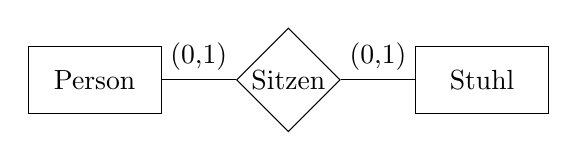
\begin{tikzpicture}[node  distance=7em]
      \node[entity] (person) {Person};
      \node[relationship] (sitzen) [right of=person] {Sitzen} edge node[above]{(0,1)} (person);
      \node[entity] (stuhl) [right of=sitzen] {Stuhl} edge node[above]{(0,1)} (sitzen);
    \end{tikzpicture}
  \end{figure}

  \todo[inline]{ggf.~zitieren: Datenmodelle, Datenbanksprachen und Datenbankmanagementsysteme
  von Gottfried Vossen}
  \todo[inline]{ERM als Thema zu allgemein? Nicht zum Seiten füllen!}

  \subsection{Dimensions-Modell}
  Es gibt verschiedene Ausprägungen des Dimensions-Modell. Zunächst wird auf
  allgemeine Eigenschaften der Modell-Gruppe eingegangen:

  Im Mittelpunkt der Dimensions-Modellierung stehen die
  betriebswirtschaftlichen \textbf{Fakten}~\cite[][S.  2]{phipps2002automating}. Ein
  Fakt kann eine Transaktion, ein Objekt oder ein Ereignis sein\cite[][S.
  42]{ballard1998data}. \citeauthor{Kemper2010} nennt als Beispiele:
  \glqq{}Umsatzerlöse, Umsatzmengen, Einzelkosten oder den
  Personalbedarf\grqq{}\cite[][S. 66]{Kemper2010}. 
  
  Um verschiedene Sichten auf diese Fakten zu erlangen gruppiert man diese in
  \textbf{Dimensionen} \bzw weist sie Dimensionsausprägungen zu~\cite[][S.
  66]{Kemper2010}. Dies ermöglicht es in der späteren Analyse nach
  verschiedenen Dimensionen zu filtern und zu vergleichen. Dimensionen werden
  hierarchisch strukturiert. Mit Hilfe der daraus entstehenden \textbf{Hierariestufen}
  kann die Sicht auf die Daten in ihrem Detailgrad angepasst werden~\cite[][S.
  66]{Kemper2010}. Wege innerhalb der Hierarchiestufen verlaufen nicht nur als
  einzelner Pfad linear, sondern auch als Baumstruktur. Ein Beispiel ist die
  Dimension \textit{Zeit}.  Diese kann zum einen durch die
  Hierarchiestufenreihe \textit{Jahr, Monat, Tag} als auch durch \textit{Jahr,
  Woche, Tag} strukturiert werden.

  Die Dimensions-Modellierung unterteit sich nun in verschiedene Ausprägungen.
  Die bekannteste Ausprägung ist das Star-Modell~\cite[][S.
  2]{phipps2002automating}. Der Name ist zurück auf den Aufbau eines
  entsprechenden Modells zu f\"uren, welcher die Form eines Sterns hat~\cite[][S.
  44]{Kimball2013}.

  Laut \textsc{\citeauthor{phipps2002automating}} wird im Umgang mit
  \acrshort{OLTP}-Systemen überwiegend auf die ER-Modellierung zurück gegriffen, wo
  hingegen \acrshort{OLAP}-Systeme meist mit der Dimensions-Modellierung konzipiert
  werden~\cite[][S. 2]{phipps2002automating}.


  \section{Existierende Methoden und Sprachen zur Analyse von Unternehmensdaten}

  \subsection{H2ForReporting}
  \subsection{Cognos}
  \subsection{Palos}

  \subsection{IBM}
  \begin{figure}[caption={Metamodell der IBM-Dimension-Sprache}, label={fig:img01}]
    \resizebox{\columnwidth}{!}{% Graphic for TeX using PGF
% Title: /home/indenml/coding/bachelor_thesis/content/figures/IBM-dimension-modelling-language.dia
% Creator: Dia v0.97.3
% CreationDate: Sat Jul 30 11:10:55 2016
% For: indenml
% \usepackage{tikz}
% The following commands are not supported in PSTricks at present
% We define them conditionally, so when they are implemented,
% this pgf file will use them.
\ifx\du\undefined{}
  \newlength{\du}
\fi
\setlength{\du}{15\unitlength}
\begin{tikzpicture}
\pgftransformxscale{1.000000}
\pgftransformyscale{-1.000000}
\definecolor{dialinecolor}{rgb}{0.000000, 0.000000, 0.000000}
\pgfsetstrokecolor{dialinecolor}
\definecolor{dialinecolor}{rgb}{1.000000, 1.000000, 1.000000}
\pgfsetfillcolor{dialinecolor}
\definecolor{dialinecolor}{rgb}{1.000000, 1.000000, 1.000000}
\pgfsetfillcolor{dialinecolor}
\fill (46.500000\du,14.550000\du)--(46.500000\du,16.350000\du)--(49.440000\du,16.350000\du)--(49.440000\du,14.550000\du)--cycle;
\pgfsetlinewidth{0.100000\du}
\pgfsetdash{}{0pt}
\pgfsetmiterjoin
\definecolor{dialinecolor}{rgb}{0.000000, 0.000000, 0.000000}
\pgfsetstrokecolor{dialinecolor}
\draw (46.500000\du,14.550000\du)--(46.500000\du,16.350000\du)--(49.440000\du,16.350000\du)--(49.440000\du,14.550000\du)--cycle;
% setfont left to latex
\definecolor{dialinecolor}{rgb}{0.000000, 0.000000, 0.000000}
\pgfsetstrokecolor{dialinecolor}
\node at (47.970000\du,15.650000\du){Fakt};
\definecolor{dialinecolor}{rgb}{1.000000, 1.000000, 1.000000}
\pgfsetfillcolor{dialinecolor}
\fill (22.050000\du,20.450000\du)--(22.050000\du,22.250000\du)--(26.915000\du,22.250000\du)--(26.915000\du,20.450000\du)--cycle;
\pgfsetlinewidth{0.100000\du}
\pgfsetdash{}{0pt}
\pgfsetmiterjoin
\definecolor{dialinecolor}{rgb}{0.000000, 0.000000, 0.000000}
\pgfsetstrokecolor{dialinecolor}
\draw (22.050000\du,20.450000\du)--(22.050000\du,22.250000\du)--(26.915000\du,22.250000\du)--(26.915000\du,20.450000\du)--cycle;
% setfont left to latex
\definecolor{dialinecolor}{rgb}{0.000000, 0.000000, 0.000000}
\pgfsetstrokecolor{dialinecolor}
\node at (24.482500\du,21.550000\du){Dimension};
\pgfsetlinewidth{0.100000\du}
\pgfsetdash{}{0pt}
\definecolor{dialinecolor}{rgb}{1.000000, 1.000000, 1.000000}
\pgfsetfillcolor{dialinecolor}
\fill (40.750000\du,11.300000\du)--(54.525000\du,11.300000\du)--(55.125000\du,11.900000\du)--(55.125000\du,13.000000\du)--(40.750000\du,13.000000\du)--cycle;
\definecolor{dialinecolor}{rgb}{0.000000, 0.000000, 0.000000}
\pgfsetstrokecolor{dialinecolor}
\draw (40.750000\du,11.300000\du)--(54.525000\du,11.300000\du)--(55.125000\du,11.900000\du)--(55.125000\du,13.000000\du)--(40.750000\du,13.000000\du)--cycle;
\pgfsetlinewidth{0.050000\du}
\definecolor{dialinecolor}{rgb}{0.000000, 0.000000, 0.000000}
\pgfsetstrokecolor{dialinecolor}
\draw (54.525000\du,11.300000\du)--(54.525000\du,11.900000\du)--(55.125000\du,11.900000\du);
% setfont left to latex
\definecolor{dialinecolor}{rgb}{0.000000, 0.000000, 0.000000}
\pgfsetstrokecolor{dialinecolor}
\node[anchor=west] at (41.100000\du,12.545000\du){Stammdatensatz / Bewegungsdatemsazu};
\pgfsetlinewidth{0.100000\du}
\pgfsetdash{}{0pt}
\pgfsetmiterjoin
\pgfsetbuttcap
\definecolor{dialinecolor}{rgb}{0.000000, 0.000000, 0.000000}
\pgfsetstrokecolor{dialinecolor}
\draw (47.937500\du,13.000000\du)--(47.937500\du,13.775000\du)--(47.970000\du,13.775000\du)--(47.970000\du,14.550000\du);
\definecolor{dialinecolor}{rgb}{1.000000, 1.000000, 1.000000}
\pgfsetfillcolor{dialinecolor}
\fill (33.600000\du,20.450000\du)--(33.600000\du,22.250000\du)--(41.545000\du,22.250000\du)--(41.545000\du,20.450000\du)--cycle;
\pgfsetlinewidth{0.100000\du}
\pgfsetdash{}{0pt}
\pgfsetmiterjoin
\definecolor{dialinecolor}{rgb}{0.000000, 0.000000, 0.000000}
\pgfsetstrokecolor{dialinecolor}
\draw (33.600000\du,20.450000\du)--(33.600000\du,22.250000\du)--(41.545000\du,22.250000\du)--(41.545000\du,20.450000\du)--cycle;
% setfont left to latex
\definecolor{dialinecolor}{rgb}{0.000000, 0.000000, 0.000000}
\pgfsetstrokecolor{dialinecolor}
\node at (37.572500\du,21.550000\du){Dimensionselement};
\definecolor{dialinecolor}{rgb}{1.000000, 1.000000, 1.000000}
\pgfsetfillcolor{dialinecolor}
\fill (29.250000\du,21.350000\du)--(30.250000\du,20.750000\du)--(31.250000\du,21.350000\du)--(30.250000\du,21.950000\du)--cycle;
\pgfsetlinewidth{0.100000\du}
\pgfsetdash{}{0pt}
\pgfsetmiterjoin
\definecolor{dialinecolor}{rgb}{0.000000, 0.000000, 0.000000}
\pgfsetstrokecolor{dialinecolor}
\draw (29.250000\du,21.350000\du)--(30.250000\du,20.750000\du)--(31.250000\du,21.350000\du)--(30.250000\du,21.950000\du)--cycle;
% setfont left to latex
\definecolor{dialinecolor}{rgb}{0.000000, 0.000000, 0.000000}
\pgfsetstrokecolor{dialinecolor}
\node[anchor=east] at (28.950000\du,21.050000\du){(0,n)};
\definecolor{dialinecolor}{rgb}{0.000000, 0.000000, 0.000000}
\pgfsetstrokecolor{dialinecolor}
\node[anchor=west] at (31.550000\du,21.050000\du){(0,1)};
\definecolor{dialinecolor}{rgb}{0.000000, 0.000000, 0.000000}
\pgfsetstrokecolor{dialinecolor}
\node at (30.250000\du,21.550000\du){};
\pgfsetlinewidth{0.100000\du}
\pgfsetdash{}{0pt}
\pgfsetmiterjoin
\pgfsetbuttcap
\definecolor{dialinecolor}{rgb}{0.000000, 0.000000, 0.000000}
\pgfsetstrokecolor{dialinecolor}
\draw (26.915000\du,21.350000\du)--(26.965000\du,21.350000\du)--(29.200000\du,21.350000\du)--(29.250000\du,21.350000\du);
\pgfsetlinewidth{0.100000\du}
\pgfsetdash{}{0pt}
\pgfsetmiterjoin
\pgfsetbuttcap
\definecolor{dialinecolor}{rgb}{0.000000, 0.000000, 0.000000}
\pgfsetstrokecolor{dialinecolor}
\draw (31.250000\du,21.350000\du)--(31.300000\du,21.350000\du)--(33.550000\du,21.350000\du)--(33.600000\du,21.350000\du);
\definecolor{dialinecolor}{rgb}{1.000000, 1.000000, 1.000000}
\pgfsetfillcolor{dialinecolor}
\fill (19.950000\du,26.350000\du)--(19.950000\du,28.150000\du)--(29.050000\du,28.150000\du)--(29.050000\du,26.350000\du)--cycle;
\pgfsetlinewidth{0.100000\du}
\pgfsetdash{}{0pt}
\pgfsetmiterjoin
\definecolor{dialinecolor}{rgb}{0.000000, 0.000000, 0.000000}
\pgfsetstrokecolor{dialinecolor}
\draw (19.950000\du,26.350000\du)--(19.950000\du,28.150000\du)--(29.050000\du,28.150000\du)--(29.050000\du,26.350000\du)--cycle;
% setfont left to latex
\definecolor{dialinecolor}{rgb}{0.000000, 0.000000, 0.000000}
\pgfsetstrokecolor{dialinecolor}
\node at (24.500000\du,27.450000\du){Dimensionshierarchie};
\definecolor{dialinecolor}{rgb}{1.000000, 1.000000, 1.000000}
\pgfsetfillcolor{dialinecolor}
\fill (23.500000\du,24.050000\du)--(24.500000\du,23.450000\du)--(25.500000\du,24.050000\du)--(24.500000\du,24.650000\du)--cycle;
\pgfsetlinewidth{0.100000\du}
\pgfsetdash{}{0pt}
\pgfsetmiterjoin
\definecolor{dialinecolor}{rgb}{0.000000, 0.000000, 0.000000}
\pgfsetstrokecolor{dialinecolor}
\draw (23.500000\du,24.050000\du)--(24.500000\du,23.450000\du)--(25.500000\du,24.050000\du)--(24.500000\du,24.650000\du)--cycle;
% setfont left to latex
\definecolor{dialinecolor}{rgb}{0.000000, 0.000000, 0.000000}
\pgfsetstrokecolor{dialinecolor}
\node[anchor=west] at (24.700000\du,23.150000\du){(0,n)};
\definecolor{dialinecolor}{rgb}{0.000000, 0.000000, 0.000000}
\pgfsetstrokecolor{dialinecolor}
\node[anchor=west] at (24.700000\du,25.750000\du){(0,1)};
\definecolor{dialinecolor}{rgb}{0.000000, 0.000000, 0.000000}
\pgfsetstrokecolor{dialinecolor}
\node at (24.500000\du,24.250000\du){};
\pgfsetlinewidth{0.100000\du}
\pgfsetdash{}{0pt}
\pgfsetmiterjoin
\pgfsetbuttcap
\definecolor{dialinecolor}{rgb}{0.000000, 0.000000, 0.000000}
\pgfsetstrokecolor{dialinecolor}
\draw (24.482500\du,22.250000\du)--(24.482500\du,22.850000\du)--(24.500000\du,22.850000\du)--(24.500000\du,23.450000\du);
\pgfsetlinewidth{0.100000\du}
\pgfsetdash{}{0pt}
\pgfsetmiterjoin
\pgfsetbuttcap
\definecolor{dialinecolor}{rgb}{0.000000, 0.000000, 0.000000}
\pgfsetstrokecolor{dialinecolor}
\draw (24.500000\du,24.650000\du)--(24.500000\du,24.700000\du)--(24.500000\du,26.300000\du)--(24.500000\du,26.350000\du);
\definecolor{dialinecolor}{rgb}{1.000000, 1.000000, 1.000000}
\pgfsetfillcolor{dialinecolor}
\fill (36.050000\du,26.350000\du)--(36.050000\du,28.150000\du)--(42.455000\du,28.150000\du)--(42.455000\du,26.350000\du)--cycle;
\pgfsetlinewidth{0.100000\du}
\pgfsetdash{}{0pt}
\pgfsetmiterjoin
\definecolor{dialinecolor}{rgb}{0.000000, 0.000000, 0.000000}
\pgfsetstrokecolor{dialinecolor}
\draw (36.050000\du,26.350000\du)--(36.050000\du,28.150000\du)--(42.455000\du,28.150000\du)--(42.455000\du,26.350000\du)--cycle;
% setfont left to latex
\definecolor{dialinecolor}{rgb}{0.000000, 0.000000, 0.000000}
\pgfsetstrokecolor{dialinecolor}
\node at (39.252500\du,27.450000\du){Hierarielevel};
\definecolor{dialinecolor}{rgb}{1.000000, 1.000000, 1.000000}
\pgfsetfillcolor{dialinecolor}
\fill (31.300000\du,27.250000\du)--(32.300000\du,26.650000\du)--(33.300000\du,27.250000\du)--(32.300000\du,27.850000\du)--cycle;
\pgfsetlinewidth{0.100000\du}
\pgfsetdash{}{0pt}
\pgfsetmiterjoin
\definecolor{dialinecolor}{rgb}{0.000000, 0.000000, 0.000000}
\pgfsetstrokecolor{dialinecolor}
\draw (31.300000\du,27.250000\du)--(32.300000\du,26.650000\du)--(33.300000\du,27.250000\du)--(32.300000\du,27.850000\du)--cycle;
% setfont left to latex
\definecolor{dialinecolor}{rgb}{0.000000, 0.000000, 0.000000}
\pgfsetstrokecolor{dialinecolor}
\node[anchor=east] at (31.000000\du,26.950000\du){(0,n)};
\definecolor{dialinecolor}{rgb}{0.000000, 0.000000, 0.000000}
\pgfsetstrokecolor{dialinecolor}
\node[anchor=west] at (33.600000\du,26.950000\du){(0,n)};
\definecolor{dialinecolor}{rgb}{0.000000, 0.000000, 0.000000}
\pgfsetstrokecolor{dialinecolor}
\node at (32.300000\du,27.450000\du){};
\pgfsetlinewidth{0.100000\du}
\pgfsetdash{}{0pt}
\pgfsetmiterjoin
\pgfsetbuttcap
\definecolor{dialinecolor}{rgb}{0.000000, 0.000000, 0.000000}
\pgfsetstrokecolor{dialinecolor}
\draw (33.300000\du,27.250000\du)--(33.350000\du,27.250000\du)--(36.000000\du,27.250000\du)--(36.050000\du,27.250000\du);
\pgfsetlinewidth{0.100000\du}
\pgfsetdash{}{0pt}
\pgfsetmiterjoin
\pgfsetbuttcap
\definecolor{dialinecolor}{rgb}{0.000000, 0.000000, 0.000000}
\pgfsetstrokecolor{dialinecolor}
\draw (31.300000\du,27.250000\du)--(31.250000\du,27.250000\du)--(29.100000\du,27.250000\du)--(29.050000\du,27.250000\du);
\pgfsetlinewidth{0.100000\du}
\pgfsetdash{}{0pt}
\definecolor{dialinecolor}{rgb}{1.000000, 1.000000, 1.000000}
\pgfsetfillcolor{dialinecolor}
\fill (24.900000\du,29.200000\du)--(39.060000\du,29.200000\du)--(39.660000\du,29.800000\du)--(39.660000\du,32.500000\du)--(24.900000\du,32.500000\du)--cycle;
\definecolor{dialinecolor}{rgb}{0.000000, 0.000000, 0.000000}
\pgfsetstrokecolor{dialinecolor}
\draw (24.900000\du,29.200000\du)--(39.060000\du,29.200000\du)--(39.660000\du,29.800000\du)--(39.660000\du,32.500000\du)--(24.900000\du,32.500000\du)--cycle;
\pgfsetlinewidth{0.050000\du}
\definecolor{dialinecolor}{rgb}{0.000000, 0.000000, 0.000000}
\pgfsetstrokecolor{dialinecolor}
\draw (39.060000\du,29.200000\du)--(39.060000\du,29.800000\du)--(39.660000\du,29.800000\du);
% setfont left to latex
\definecolor{dialinecolor}{rgb}{0.000000, 0.000000, 0.000000}
\pgfsetstrokecolor{dialinecolor}
\node[anchor=west] at (25.250000\du,30.445000\du){Tag kann sowohl in der Hierarchie };
% setfont left to latex
\definecolor{dialinecolor}{rgb}{0.000000, 0.000000, 0.000000}
\pgfsetstrokecolor{dialinecolor}
\node[anchor=west] at (25.250000\du,31.245000\du){Jahr|Monat|Tag als auch in Woche|Tag};
% setfont left to latex
\definecolor{dialinecolor}{rgb}{0.000000, 0.000000, 0.000000}
\pgfsetstrokecolor{dialinecolor}
\node[anchor=west] at (25.250000\du,32.045000\du){vorkommen};
\pgfsetlinewidth{0.100000\du}
\pgfsetdash{}{0pt}
\pgfsetmiterjoin
\pgfsetbuttcap
\definecolor{dialinecolor}{rgb}{0.000000, 0.000000, 0.000000}
\pgfsetstrokecolor{dialinecolor}
\draw (32.280000\du,29.200000\du)--(32.280000\du,28.525000\du)--(32.300000\du,28.525000\du)--(32.300000\du,27.850000\du);
\definecolor{dialinecolor}{rgb}{1.000000, 1.000000, 1.000000}
\pgfsetfillcolor{dialinecolor}
\fill (54.300000\du,20.450000\du)--(54.300000\du,22.250000\du)--(58.780000\du,22.250000\du)--(58.780000\du,20.450000\du)--cycle;
\pgfsetlinewidth{0.100000\du}
\pgfsetdash{}{0pt}
\pgfsetmiterjoin
\definecolor{dialinecolor}{rgb}{0.000000, 0.000000, 0.000000}
\pgfsetstrokecolor{dialinecolor}
\draw (54.300000\du,20.450000\du)--(54.300000\du,22.250000\du)--(58.780000\du,22.250000\du)--(58.780000\du,20.450000\du)--cycle;
% setfont left to latex
\definecolor{dialinecolor}{rgb}{0.000000, 0.000000, 0.000000}
\pgfsetstrokecolor{dialinecolor}
\node at (56.540000\du,21.550000\du){Kennzahl};
\definecolor{dialinecolor}{rgb}{1.000000, 1.000000, 1.000000}
\pgfsetfillcolor{dialinecolor}
\fill (44.750000\du,21.370500\du)--(47.867500\du,19.500000\du)--(50.985000\du,21.370500\du)--(47.867500\du,23.241000\du)--cycle;
\pgfsetlinewidth{0.100000\du}
\pgfsetdash{}{0pt}
\pgfsetmiterjoin
\definecolor{dialinecolor}{rgb}{0.000000, 0.000000, 0.000000}
\pgfsetstrokecolor{dialinecolor}
\draw (44.750000\du,21.370500\du)--(47.867500\du,19.500000\du)--(50.985000\du,21.370500\du)--(47.867500\du,23.241000\du)--cycle;
% setfont left to latex
\definecolor{dialinecolor}{rgb}{0.000000, 0.000000, 0.000000}
\pgfsetstrokecolor{dialinecolor}
\node[anchor=east] at (44.450000\du,21.070500\du){(0,n)};
\definecolor{dialinecolor}{rgb}{0.000000, 0.000000, 0.000000}
\pgfsetstrokecolor{dialinecolor}
\node[anchor=west] at (51.285000\du,21.070500\du){(0,n)};
\definecolor{dialinecolor}{rgb}{0.000000, 0.000000, 0.000000}
\pgfsetstrokecolor{dialinecolor}
\node at (47.867500\du,21.570500\du){Kombination};
\pgfsetlinewidth{0.100000\du}
\pgfsetdash{}{0pt}
\pgfsetmiterjoin
\pgfsetbuttcap
\definecolor{dialinecolor}{rgb}{0.000000, 0.000000, 0.000000}
\pgfsetstrokecolor{dialinecolor}
\draw (41.545000\du,21.350000\du)--(43.147500\du,21.350000\du)--(43.147500\du,21.370500\du)--(44.750000\du,21.370500\du);
\pgfsetlinewidth{0.100000\du}
\pgfsetdash{}{0pt}
\pgfsetmiterjoin
\pgfsetbuttcap
\definecolor{dialinecolor}{rgb}{0.000000, 0.000000, 0.000000}
\pgfsetstrokecolor{dialinecolor}
\draw (50.985000\du,21.370500\du)--(52.642500\du,21.370500\du)--(52.642500\du,21.350000\du)--(54.300000\du,21.350000\du);
\definecolor{dialinecolor}{rgb}{1.000000, 1.000000, 1.000000}
\pgfsetfillcolor{dialinecolor}
\fill (51.950000\du,15.450000\du)--(52.950000\du,14.850000\du)--(53.950000\du,15.450000\du)--(52.950000\du,16.050000\du)--cycle;
\pgfsetlinewidth{0.100000\du}
\pgfsetdash{}{0pt}
\pgfsetmiterjoin
\definecolor{dialinecolor}{rgb}{0.000000, 0.000000, 0.000000}
\pgfsetstrokecolor{dialinecolor}
\draw (51.950000\du,15.450000\du)--(52.950000\du,14.850000\du)--(53.950000\du,15.450000\du)--(52.950000\du,16.050000\du)--cycle;
% setfont left to latex
\definecolor{dialinecolor}{rgb}{0.000000, 0.000000, 0.000000}
\pgfsetstrokecolor{dialinecolor}
\node[anchor=east] at (51.650000\du,15.150000\du){(0,n)};
\definecolor{dialinecolor}{rgb}{0.000000, 0.000000, 0.000000}
\pgfsetstrokecolor{dialinecolor}
\node[anchor=west] at (54.250000\du,15.150000\du){(0,n)};
\definecolor{dialinecolor}{rgb}{0.000000, 0.000000, 0.000000}
\pgfsetstrokecolor{dialinecolor}
\node at (52.950000\du,15.650000\du){};
\pgfsetlinewidth{0.100000\du}
\pgfsetdash{}{0pt}
\pgfsetmiterjoin
\pgfsetbuttcap
\definecolor{dialinecolor}{rgb}{0.000000, 0.000000, 0.000000}
\pgfsetstrokecolor{dialinecolor}
\draw (53.950000\du,15.450000\du)--(53.950000\du,15.500000\du)--(56.540000\du,15.500000\du)--(56.540000\du,20.450000\du);
\pgfsetlinewidth{0.100000\du}
\pgfsetdash{}{0pt}
\pgfsetmiterjoin
\pgfsetbuttcap
\definecolor{dialinecolor}{rgb}{0.000000, 0.000000, 0.000000}
\pgfsetstrokecolor{dialinecolor}
\draw (49.440000\du,15.450000\du)--(49.490000\du,15.450000\du)--(51.900000\du,15.450000\du)--(51.950000\du,15.450000\du);
\definecolor{dialinecolor}{rgb}{1.000000, 1.000000, 1.000000}
\pgfsetfillcolor{dialinecolor}
\fill (35.950000\du,14.550000\du)--(35.950000\du,16.350000\du)--(39.275000\du,16.350000\du)--(39.275000\du,14.550000\du)--cycle;
\pgfsetlinewidth{0.100000\du}
\pgfsetdash{}{0pt}
\pgfsetmiterjoin
\definecolor{dialinecolor}{rgb}{0.000000, 0.000000, 0.000000}
\pgfsetstrokecolor{dialinecolor}
\draw (35.950000\du,14.550000\du)--(35.950000\du,16.350000\du)--(39.275000\du,16.350000\du)--(39.275000\du,14.550000\du)--cycle;
% setfont left to latex
\definecolor{dialinecolor}{rgb}{0.000000, 0.000000, 0.000000}
\pgfsetstrokecolor{dialinecolor}
\node at (37.612500\du,15.650000\du){Datum};
\definecolor{dialinecolor}{rgb}{1.000000, 1.000000, 1.000000}
\pgfsetfillcolor{dialinecolor}
\fill (41.500000\du,15.450000\du)--(42.500000\du,14.850000\du)--(43.500000\du,15.450000\du)--(42.500000\du,16.050000\du)--cycle;
\pgfsetlinewidth{0.100000\du}
\pgfsetdash{}{0pt}
\pgfsetmiterjoin
\definecolor{dialinecolor}{rgb}{0.000000, 0.000000, 0.000000}
\pgfsetstrokecolor{dialinecolor}
\draw (41.500000\du,15.450000\du)--(42.500000\du,14.850000\du)--(43.500000\du,15.450000\du)--(42.500000\du,16.050000\du)--cycle;
% setfont left to latex
\definecolor{dialinecolor}{rgb}{0.000000, 0.000000, 0.000000}
\pgfsetstrokecolor{dialinecolor}
\node[anchor=east] at (41.200000\du,15.150000\du){(0,1)};
\definecolor{dialinecolor}{rgb}{0.000000, 0.000000, 0.000000}
\pgfsetstrokecolor{dialinecolor}
\node[anchor=west] at (43.800000\du,15.150000\du){(0,n)};
\definecolor{dialinecolor}{rgb}{0.000000, 0.000000, 0.000000}
\pgfsetstrokecolor{dialinecolor}
\node at (42.500000\du,15.650000\du){};
\pgfsetlinewidth{0.100000\du}
\pgfsetdash{}{0pt}
\pgfsetmiterjoin
\pgfsetbuttcap
\definecolor{dialinecolor}{rgb}{0.000000, 0.000000, 0.000000}
\pgfsetstrokecolor{dialinecolor}
\draw (39.275000\du,15.450000\du)--(39.325000\du,15.450000\du)--(41.450000\du,15.450000\du)--(41.500000\du,15.450000\du);
\pgfsetlinewidth{0.100000\du}
\pgfsetdash{}{0pt}
\pgfsetmiterjoin
\pgfsetbuttcap
\definecolor{dialinecolor}{rgb}{0.000000, 0.000000, 0.000000}
\pgfsetstrokecolor{dialinecolor}
\draw (43.500000\du,15.450000\du)--(43.550000\du,15.450000\du)--(46.450000\du,15.450000\du)--(46.500000\du,15.450000\du);
\definecolor{dialinecolor}{rgb}{1.000000, 1.000000, 1.000000}
\pgfsetfillcolor{dialinecolor}
\fill (36.600000\du,18.450000\du)--(37.600000\du,17.850000\du)--(38.600000\du,18.450000\du)--(37.600000\du,19.050000\du)--cycle;
\pgfsetlinewidth{0.100000\du}
\pgfsetdash{}{0pt}
\pgfsetmiterjoin
\definecolor{dialinecolor}{rgb}{0.000000, 0.000000, 0.000000}
\pgfsetstrokecolor{dialinecolor}
\draw (36.600000\du,18.450000\du)--(37.600000\du,17.850000\du)--(38.600000\du,18.450000\du)--(37.600000\du,19.050000\du)--cycle;
% setfont left to latex
\definecolor{dialinecolor}{rgb}{0.000000, 0.000000, 0.000000}
\pgfsetstrokecolor{dialinecolor}
\node[anchor=west] at (37.800000\du,17.550000\du){(1,1)};
\definecolor{dialinecolor}{rgb}{0.000000, 0.000000, 0.000000}
\pgfsetstrokecolor{dialinecolor}
\node[anchor=west] at (37.800000\du,20.150000\du){(0,n)};
\definecolor{dialinecolor}{rgb}{0.000000, 0.000000, 0.000000}
\pgfsetstrokecolor{dialinecolor}
\node at (37.600000\du,18.650000\du){};
\pgfsetlinewidth{0.100000\du}
\pgfsetdash{}{0pt}
\pgfsetmiterjoin
\pgfsetbuttcap
\definecolor{dialinecolor}{rgb}{0.000000, 0.000000, 0.000000}
\pgfsetstrokecolor{dialinecolor}
\draw (37.600000\du,19.050000\du)--(37.600000\du,19.750000\du)--(37.572500\du,19.750000\du)--(37.572500\du,20.450000\du);
\pgfsetlinewidth{0.100000\du}
\pgfsetdash{}{0pt}
\pgfsetmiterjoin
\pgfsetbuttcap
\definecolor{dialinecolor}{rgb}{0.000000, 0.000000, 0.000000}
\pgfsetstrokecolor{dialinecolor}
\draw (37.600000\du,17.850000\du)--(37.600000\du,17.100000\du)--(37.612500\du,17.100000\du)--(37.612500\du,16.350000\du);
\end{tikzpicture}
}
  \end{figure}
  Zwei Methoden



  \section{Beispielszenario}
  Für den weiteren Verlauf dieser Arbeit wird ein Beispielszenario aufgestellt. Im
  Fokus steht eine fiktive Firma namens SmartSell. SmartSell setzt seine
  Produkte sowohl klassisch über ihr lokales Geschäft, als auch über einen
  eigenen Online-Shop ab.

  Beispiel Dimensionen
  \begin{itemize}
    \item Absatzkanal
    \item Zeit
    \item Produkt
    \item Ort
    \item Kunde
    \item Personal
    \item Lieferant
    \item Wertansatz (Soll, Ist, Plan)
  \end{itemize}

  \section{Rahmenbedingungen und Annahmen}
  \begin{itemize}
    \item Input Daten voll normalisiert
    \item Star-Schema denormalisiert
    \item Snow-Schema normalisiert
  \end{itemize}

  % ################################################################################
  \chapter{DataFurnace-Sprache für innoscale}
  % ################################################################################

  \texthl{Ein Subset von H2ForReporting? F\"ur DQM statt f\"ur Business Intelligence?}

  \section{Sprache}
  \begin{figure}[caption={Metamodell der DataFurnace-Sprache}, label={fig:img01}]
    \resizebox{\columnwidth}{!}{% Graphic for TeX using PGF
% Title: /home/indenml/code/bachelor_thesis/content/figures/language_spec-erm.dia
% Creator: Dia v0.97.3
% CreationDate: Tue Sep 27 11:28:12 2016
% For: indenml
% \usepackage{tikz}
% The following commands are not supported in PSTricks at present
% We define them conditionally, so when they are implemented,
% this pgf file will use them.
\ifx\du\undefined
  \newlength{\du}
\fi
\setlength{\du}{15\unitlength}
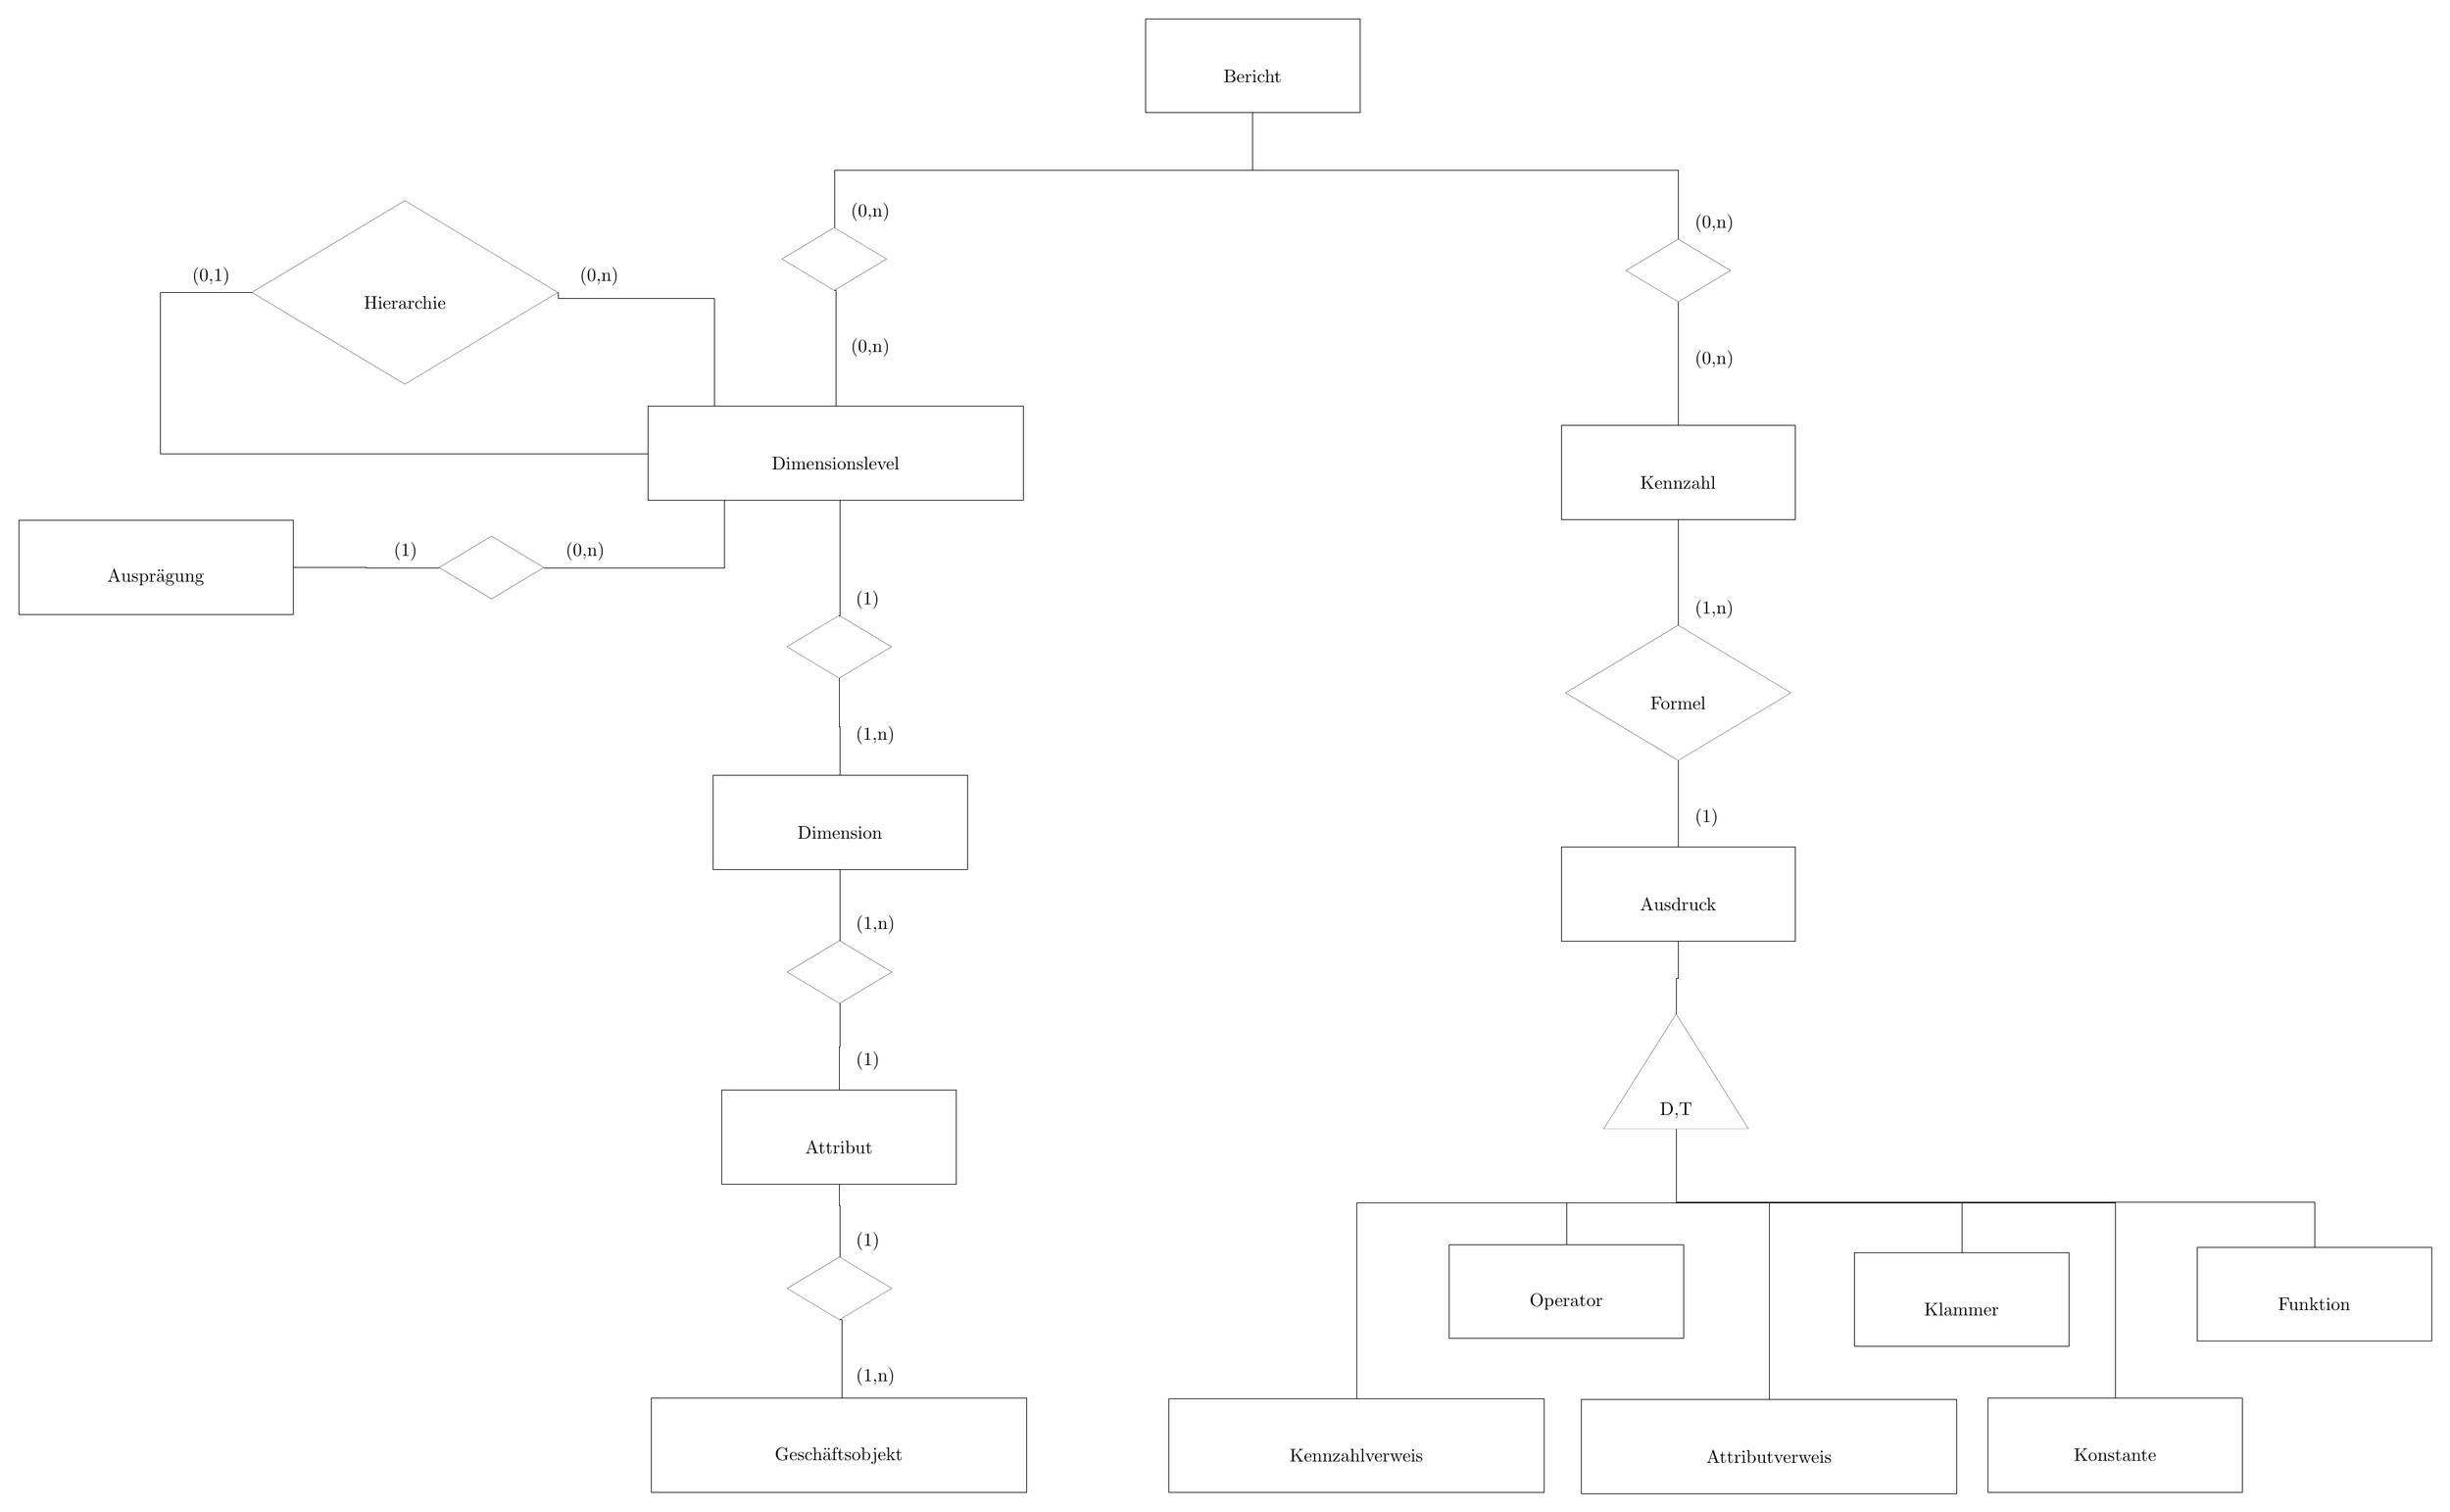
\begin{tikzpicture}
\pgftransformxscale{1.000000}
\pgftransformyscale{-1.000000}
\definecolor{dialinecolor}{rgb}{0.000000, 0.000000, 0.000000}
\pgfsetstrokecolor{dialinecolor}
\definecolor{dialinecolor}{rgb}{1.000000, 1.000000, 1.000000}
\pgfsetfillcolor{dialinecolor}
\definecolor{dialinecolor}{rgb}{1.000000, 1.000000, 1.000000}
\pgfsetfillcolor{dialinecolor}
\fill (-1.973220\du,32.336600\du)--(-1.973220\du,34.136600\du)--(2.891780\du,34.136600\du)--(2.891780\du,32.336600\du)--cycle;
\pgfsetlinewidth{0.100000\du}
\pgfsetdash{}{0pt}
\pgfsetmiterjoin
\definecolor{dialinecolor}{rgb}{0.000000, 0.000000, 0.000000}
\pgfsetstrokecolor{dialinecolor}
\draw (-1.973220\du,32.336600\du)--(-1.973220\du,34.136600\du)--(2.891780\du,34.136600\du)--(2.891780\du,32.336600\du)--cycle;
% setfont left to latex
\definecolor{dialinecolor}{rgb}{0.000000, 0.000000, 0.000000}
\pgfsetstrokecolor{dialinecolor}
\node at (0.459280\du,33.436600\du){Dimension};
\definecolor{dialinecolor}{rgb}{1.000000, 1.000000, 1.000000}
\pgfsetfillcolor{dialinecolor}
\fill (-3.210480\du,25.273700\du)--(-3.210480\du,27.073700\du)--(3.964520\du,27.073700\du)--(3.964520\du,25.273700\du)--cycle;
\pgfsetlinewidth{0.100000\du}
\pgfsetdash{}{0pt}
\pgfsetmiterjoin
\definecolor{dialinecolor}{rgb}{0.000000, 0.000000, 0.000000}
\pgfsetstrokecolor{dialinecolor}
\draw (-3.210480\du,25.273700\du)--(-3.210480\du,27.073700\du)--(3.964520\du,27.073700\du)--(3.964520\du,25.273700\du)--cycle;
% setfont left to latex
\definecolor{dialinecolor}{rgb}{0.000000, 0.000000, 0.000000}
\pgfsetstrokecolor{dialinecolor}
\node at (0.377020\du,26.373700\du){Dimensionslevel};
\definecolor{dialinecolor}{rgb}{1.000000, 1.000000, 1.000000}
\pgfsetfillcolor{dialinecolor}
\fill (-1.800000\du,38.350000\du)--(-1.800000\du,40.150000\du)--(2.680000\du,40.150000\du)--(2.680000\du,38.350000\du)--cycle;
\pgfsetlinewidth{0.100000\du}
\pgfsetdash{}{0pt}
\pgfsetmiterjoin
\definecolor{dialinecolor}{rgb}{0.000000, 0.000000, 0.000000}
\pgfsetstrokecolor{dialinecolor}
\draw (-1.800000\du,38.350000\du)--(-1.800000\du,40.150000\du)--(2.680000\du,40.150000\du)--(2.680000\du,38.350000\du)--cycle;
% setfont left to latex
\definecolor{dialinecolor}{rgb}{0.000000, 0.000000, 0.000000}
\pgfsetstrokecolor{dialinecolor}
\node at (0.440000\du,39.450000\du){Attribut};
\definecolor{dialinecolor}{rgb}{1.000000, 1.000000, 1.000000}
\pgfsetfillcolor{dialinecolor}
\fill (-10.782700\du,23.101400\du)--(-7.857700\du,21.346400\du)--(-4.932700\du,23.101400\du)--(-7.857700\du,24.856400\du)--cycle;
\pgfsetlinewidth{0.100000\du}
\pgfsetdash{}{0pt}
\pgfsetmiterjoin
\definecolor{dialinecolor}{rgb}{0.000000, 0.000000, 0.000000}
\pgfsetstrokecolor{dialinecolor}
\draw (-10.782700\du,23.101400\du)--(-7.857700\du,21.346400\du)--(-4.932700\du,23.101400\du)--(-7.857700\du,24.856400\du)--cycle;
% setfont left to latex
\definecolor{dialinecolor}{rgb}{0.000000, 0.000000, 0.000000}
\pgfsetstrokecolor{dialinecolor}
\node[anchor=east] at (-11.082700\du,22.801400\du){(0,1)};
\definecolor{dialinecolor}{rgb}{0.000000, 0.000000, 0.000000}
\pgfsetstrokecolor{dialinecolor}
\node[anchor=west] at (-4.632700\du,22.801400\du){(0,n)};
\definecolor{dialinecolor}{rgb}{0.000000, 0.000000, 0.000000}
\pgfsetstrokecolor{dialinecolor}
\node at (-7.857700\du,23.301400\du){Hierarchie};
\pgfsetlinewidth{0.100000\du}
\pgfsetdash{}{0pt}
\pgfsetmiterjoin
\pgfsetbuttcap
\definecolor{dialinecolor}{rgb}{0.000000, 0.000000, 0.000000}
\pgfsetstrokecolor{dialinecolor}
\draw (-3.210480\du,26.173700\du)--(-3.210480\du,26.182300\du)--(-12.537500\du,26.182300\du)--(-12.537500\du,23.101400\du)--(-10.782700\du,23.101400\du);
\pgfsetlinewidth{0.100000\du}
\pgfsetdash{}{0pt}
\pgfsetmiterjoin
\pgfsetbuttcap
\definecolor{dialinecolor}{rgb}{0.000000, 0.000000, 0.000000}
\pgfsetstrokecolor{dialinecolor}
\draw (0.377020\du,25.273700\du)--(-1.943990\du,25.273700\du)--(-1.943990\du,23.212500\du)--(-4.932700\du,23.212500\du)--(-4.932700\du,23.101400\du);
\definecolor{dialinecolor}{rgb}{1.000000, 1.000000, 1.000000}
\pgfsetfillcolor{dialinecolor}
\fill (-0.555025\du,29.879100\du)--(0.444975\du,29.279100\du)--(1.444975\du,29.879100\du)--(0.444975\du,30.479100\du)--cycle;
\pgfsetlinewidth{0.100000\du}
\pgfsetdash{}{0pt}
\pgfsetmiterjoin
\definecolor{dialinecolor}{rgb}{0.000000, 0.000000, 0.000000}
\pgfsetstrokecolor{dialinecolor}
\draw (-0.555025\du,29.879100\du)--(0.444975\du,29.279100\du)--(1.444975\du,29.879100\du)--(0.444975\du,30.479100\du)--cycle;
% setfont left to latex
\definecolor{dialinecolor}{rgb}{0.000000, 0.000000, 0.000000}
\pgfsetstrokecolor{dialinecolor}
\node[anchor=west] at (0.644975\du,28.979100\du){(1) };
\definecolor{dialinecolor}{rgb}{0.000000, 0.000000, 0.000000}
\pgfsetstrokecolor{dialinecolor}
\node[anchor=west] at (0.644975\du,31.579100\du){(1,n) };
\definecolor{dialinecolor}{rgb}{0.000000, 0.000000, 0.000000}
\pgfsetstrokecolor{dialinecolor}
\node at (0.444975\du,30.079100\du){};
\pgfsetlinewidth{0.100000\du}
\pgfsetdash{}{0pt}
\pgfsetmiterjoin
\pgfsetbuttcap
\definecolor{dialinecolor}{rgb}{0.000000, 0.000000, 0.000000}
\pgfsetstrokecolor{dialinecolor}
\draw (0.459280\du,32.336600\du)--(0.459280\du,31.407850\du)--(0.444975\du,31.407850\du)--(0.444975\du,30.479100\du);
\pgfsetlinewidth{0.100000\du}
\pgfsetdash{}{0pt}
\pgfsetmiterjoin
\pgfsetbuttcap
\definecolor{dialinecolor}{rgb}{0.000000, 0.000000, 0.000000}
\pgfsetstrokecolor{dialinecolor}
\draw (0.444975\du,29.279100\du)--(0.450000\du,29.279100\du)--(0.450000\du,27.073700\du)--(0.377020\du,27.073700\du);
\definecolor{dialinecolor}{rgb}{1.000000, 1.000000, 1.000000}
\pgfsetfillcolor{dialinecolor}
\fill (-0.550000\du,36.100000\du)--(0.450000\du,35.500000\du)--(1.450000\du,36.100000\du)--(0.450000\du,36.700000\du)--cycle;
\pgfsetlinewidth{0.100000\du}
\pgfsetdash{}{0pt}
\pgfsetmiterjoin
\definecolor{dialinecolor}{rgb}{0.000000, 0.000000, 0.000000}
\pgfsetstrokecolor{dialinecolor}
\draw (-0.550000\du,36.100000\du)--(0.450000\du,35.500000\du)--(1.450000\du,36.100000\du)--(0.450000\du,36.700000\du)--cycle;
% setfont left to latex
\definecolor{dialinecolor}{rgb}{0.000000, 0.000000, 0.000000}
\pgfsetstrokecolor{dialinecolor}
\node[anchor=west] at (0.650000\du,35.200000\du){(1,n)};
\definecolor{dialinecolor}{rgb}{0.000000, 0.000000, 0.000000}
\pgfsetstrokecolor{dialinecolor}
\node[anchor=west] at (0.650000\du,37.800000\du){(1)};
\definecolor{dialinecolor}{rgb}{0.000000, 0.000000, 0.000000}
\pgfsetstrokecolor{dialinecolor}
\node at (0.450000\du,36.300000\du){};
\definecolor{dialinecolor}{rgb}{1.000000, 1.000000, 1.000000}
\pgfsetfillcolor{dialinecolor}
\fill (14.242400\du,25.644600\du)--(14.242400\du,27.444600\du)--(18.722400\du,27.444600\du)--(18.722400\du,25.644600\du)--cycle;
\pgfsetlinewidth{0.100000\du}
\pgfsetdash{}{0pt}
\pgfsetmiterjoin
\definecolor{dialinecolor}{rgb}{0.000000, 0.000000, 0.000000}
\pgfsetstrokecolor{dialinecolor}
\draw (14.242400\du,25.644600\du)--(14.242400\du,27.444600\du)--(18.722400\du,27.444600\du)--(18.722400\du,25.644600\du)--cycle;
% setfont left to latex
\definecolor{dialinecolor}{rgb}{0.000000, 0.000000, 0.000000}
\pgfsetstrokecolor{dialinecolor}
\node at (16.482400\du,26.744600\du){Kennzahl};
\definecolor{dialinecolor}{rgb}{1.000000, 1.000000, 1.000000}
\pgfsetfillcolor{dialinecolor}
\fill (14.244400\du,33.701100\du)--(14.244400\du,35.501100\du)--(18.724400\du,35.501100\du)--(18.724400\du,33.701100\du)--cycle;
\pgfsetlinewidth{0.100000\du}
\pgfsetdash{}{0pt}
\pgfsetmiterjoin
\definecolor{dialinecolor}{rgb}{0.000000, 0.000000, 0.000000}
\pgfsetstrokecolor{dialinecolor}
\draw (14.244400\du,33.701100\du)--(14.244400\du,35.501100\du)--(18.724400\du,35.501100\du)--(18.724400\du,33.701100\du)--cycle;
% setfont left to latex
\definecolor{dialinecolor}{rgb}{0.000000, 0.000000, 0.000000}
\pgfsetstrokecolor{dialinecolor}
\node at (16.484400\du,34.801100\du){Ausdruck};
\definecolor{dialinecolor}{rgb}{1.000000, 1.000000, 1.000000}
\pgfsetfillcolor{dialinecolor}
\fill (14.329000\du,30.760100\du)--(16.484000\du,29.467100\du)--(18.639000\du,30.760100\du)--(16.484000\du,32.053100\du)--cycle;
\pgfsetlinewidth{0.100000\du}
\pgfsetdash{}{0pt}
\pgfsetmiterjoin
\definecolor{dialinecolor}{rgb}{0.000000, 0.000000, 0.000000}
\pgfsetstrokecolor{dialinecolor}
\draw (14.329000\du,30.760100\du)--(16.484000\du,29.467100\du)--(18.639000\du,30.760100\du)--(16.484000\du,32.053100\du)--cycle;
% setfont left to latex
\definecolor{dialinecolor}{rgb}{0.000000, 0.000000, 0.000000}
\pgfsetstrokecolor{dialinecolor}
\node[anchor=west] at (16.684000\du,29.167100\du){(1,n)};
\definecolor{dialinecolor}{rgb}{0.000000, 0.000000, 0.000000}
\pgfsetstrokecolor{dialinecolor}
\node[anchor=west] at (16.684000\du,33.153100\du){(1)};
\definecolor{dialinecolor}{rgb}{0.000000, 0.000000, 0.000000}
\pgfsetstrokecolor{dialinecolor}
\node at (16.484000\du,30.960100\du){Formel};
\pgfsetlinewidth{0.100000\du}
\pgfsetdash{}{0pt}
\pgfsetmiterjoin
\pgfsetbuttcap
\definecolor{dialinecolor}{rgb}{0.000000, 0.000000, 0.000000}
\pgfsetstrokecolor{dialinecolor}
\draw (16.482400\du,27.444600\du)--(16.482400\du,27.437200\du)--(16.484000\du,27.437200\du)--(16.484000\du,29.467100\du);
\pgfsetlinewidth{0.100000\du}
\pgfsetdash{}{0pt}
\pgfsetmiterjoin
\pgfsetbuttcap
\definecolor{dialinecolor}{rgb}{0.000000, 0.000000, 0.000000}
\pgfsetstrokecolor{dialinecolor}
\draw (16.484000\du,32.053100\du)--(16.483900\du,32.053100\du)--(16.483900\du,33.701100\du)--(16.484400\du,33.701100\du);
\pgfsetlinewidth{0.100000\du}
\pgfsetdash{}{0pt}
\pgfsetdash{}{0pt}
\pgfsetbuttcap
\pgfsetmiterjoin
\pgfsetlinewidth{0.100000\du}
\pgfsetbuttcap
\pgfsetmiterjoin
\pgfsetdash{}{0pt}
\definecolor{dialinecolor}{rgb}{1.000000, 1.000000, 1.000000}
\pgfsetfillcolor{dialinecolor}
\fill (15.059400\du,39.100000\du)--(17.829400\du,39.100000\du)--(16.444400\du,36.900000\du)--cycle;
\definecolor{dialinecolor}{rgb}{0.000000, 0.000000, 0.000000}
\pgfsetstrokecolor{dialinecolor}
\draw (15.059400\du,39.100000\du)--(17.829400\du,39.100000\du)--(16.444400\du,36.900000\du)--cycle;
% setfont left to latex
\definecolor{dialinecolor}{rgb}{0.000000, 0.000000, 0.000000}
\pgfsetstrokecolor{dialinecolor}
\node at (16.444400\du,38.750000\du){D,T};
\definecolor{dialinecolor}{rgb}{1.000000, 1.000000, 1.000000}
\pgfsetfillcolor{dialinecolor}
\fill (26.404400\du,41.356500\du)--(26.404400\du,43.156500\du)--(30.884400\du,43.156500\du)--(30.884400\du,41.356500\du)--cycle;
\pgfsetlinewidth{0.100000\du}
\pgfsetdash{}{0pt}
\pgfsetmiterjoin
\definecolor{dialinecolor}{rgb}{0.000000, 0.000000, 0.000000}
\pgfsetstrokecolor{dialinecolor}
\draw (26.404400\du,41.356500\du)--(26.404400\du,43.156500\du)--(30.884400\du,43.156500\du)--(30.884400\du,41.356500\du)--cycle;
% setfont left to latex
\definecolor{dialinecolor}{rgb}{0.000000, 0.000000, 0.000000}
\pgfsetstrokecolor{dialinecolor}
\node at (28.644400\du,42.456500\du){Funktion};
\definecolor{dialinecolor}{rgb}{1.000000, 1.000000, 1.000000}
\pgfsetfillcolor{dialinecolor}
\fill (12.104400\du,41.306500\du)--(12.104400\du,43.106500\du)--(16.584400\du,43.106500\du)--(16.584400\du,41.306500\du)--cycle;
\pgfsetlinewidth{0.100000\du}
\pgfsetdash{}{0pt}
\pgfsetmiterjoin
\definecolor{dialinecolor}{rgb}{0.000000, 0.000000, 0.000000}
\pgfsetstrokecolor{dialinecolor}
\draw (12.104400\du,41.306500\du)--(12.104400\du,43.106500\du)--(16.584400\du,43.106500\du)--(16.584400\du,41.306500\du)--cycle;
% setfont left to latex
\definecolor{dialinecolor}{rgb}{0.000000, 0.000000, 0.000000}
\pgfsetstrokecolor{dialinecolor}
\node at (14.344400\du,42.406500\du){Operator};
\definecolor{dialinecolor}{rgb}{1.000000, 1.000000, 1.000000}
\pgfsetfillcolor{dialinecolor}
\fill (19.854400\du,41.456500\du)--(19.854400\du,43.256500\du)--(23.949400\du,43.256500\du)--(23.949400\du,41.456500\du)--cycle;
\pgfsetlinewidth{0.100000\du}
\pgfsetdash{}{0pt}
\pgfsetmiterjoin
\definecolor{dialinecolor}{rgb}{0.000000, 0.000000, 0.000000}
\pgfsetstrokecolor{dialinecolor}
\draw (19.854400\du,41.456500\du)--(19.854400\du,43.256500\du)--(23.949400\du,43.256500\du)--(23.949400\du,41.456500\du)--cycle;
% setfont left to latex
\definecolor{dialinecolor}{rgb}{0.000000, 0.000000, 0.000000}
\pgfsetstrokecolor{dialinecolor}
\node at (21.901900\du,42.556500\du){Klammer};
\definecolor{dialinecolor}{rgb}{1.000000, 1.000000, 1.000000}
\pgfsetfillcolor{dialinecolor}
\fill (6.300000\du,17.862500\du)--(6.300000\du,19.662500\du)--(10.395000\du,19.662500\du)--(10.395000\du,17.862500\du)--cycle;
\pgfsetlinewidth{0.100000\du}
\pgfsetdash{}{0pt}
\pgfsetmiterjoin
\definecolor{dialinecolor}{rgb}{0.000000, 0.000000, 0.000000}
\pgfsetstrokecolor{dialinecolor}
\draw (6.300000\du,17.862500\du)--(6.300000\du,19.662500\du)--(10.395000\du,19.662500\du)--(10.395000\du,17.862500\du)--cycle;
% setfont left to latex
\definecolor{dialinecolor}{rgb}{0.000000, 0.000000, 0.000000}
\pgfsetstrokecolor{dialinecolor}
\node at (8.347500\du,18.962500\du){Bericht};
\definecolor{dialinecolor}{rgb}{1.000000, 1.000000, 1.000000}
\pgfsetfillcolor{dialinecolor}
\fill (-0.650000\du,22.462500\du)--(0.350000\du,21.862500\du)--(1.350000\du,22.462500\du)--(0.350000\du,23.062500\du)--cycle;
\pgfsetlinewidth{0.100000\du}
\pgfsetdash{}{0pt}
\pgfsetmiterjoin
\definecolor{dialinecolor}{rgb}{0.000000, 0.000000, 0.000000}
\pgfsetstrokecolor{dialinecolor}
\draw (-0.650000\du,22.462500\du)--(0.350000\du,21.862500\du)--(1.350000\du,22.462500\du)--(0.350000\du,23.062500\du)--cycle;
% setfont left to latex
\definecolor{dialinecolor}{rgb}{0.000000, 0.000000, 0.000000}
\pgfsetstrokecolor{dialinecolor}
\node[anchor=west] at (0.550000\du,21.562500\du){(0,n)};
\definecolor{dialinecolor}{rgb}{0.000000, 0.000000, 0.000000}
\pgfsetstrokecolor{dialinecolor}
\node[anchor=west] at (0.550000\du,24.162500\du){(0,n)};
\definecolor{dialinecolor}{rgb}{0.000000, 0.000000, 0.000000}
\pgfsetstrokecolor{dialinecolor}
\node at (0.350000\du,22.662500\du){};
\definecolor{dialinecolor}{rgb}{1.000000, 1.000000, 1.000000}
\pgfsetfillcolor{dialinecolor}
\fill (15.485600\du,22.683200\du)--(16.485600\du,22.083200\du)--(17.485600\du,22.683200\du)--(16.485600\du,23.283200\du)--cycle;
\pgfsetlinewidth{0.100000\du}
\pgfsetdash{}{0pt}
\pgfsetmiterjoin
\definecolor{dialinecolor}{rgb}{0.000000, 0.000000, 0.000000}
\pgfsetstrokecolor{dialinecolor}
\draw (15.485600\du,22.683200\du)--(16.485600\du,22.083200\du)--(17.485600\du,22.683200\du)--(16.485600\du,23.283200\du)--cycle;
% setfont left to latex
\definecolor{dialinecolor}{rgb}{0.000000, 0.000000, 0.000000}
\pgfsetstrokecolor{dialinecolor}
\node[anchor=west] at (16.685600\du,21.783200\du){(0,n)};
\definecolor{dialinecolor}{rgb}{0.000000, 0.000000, 0.000000}
\pgfsetstrokecolor{dialinecolor}
\node[anchor=west] at (16.685600\du,24.383200\du){(0,n)};
\definecolor{dialinecolor}{rgb}{0.000000, 0.000000, 0.000000}
\pgfsetstrokecolor{dialinecolor}
\node at (16.485600\du,22.883200\du){};
\definecolor{dialinecolor}{rgb}{1.000000, 1.000000, 1.000000}
\pgfsetfillcolor{dialinecolor}
\fill (-7.201620\du,28.363300\du)--(-6.201620\du,27.763300\du)--(-5.201620\du,28.363300\du)--(-6.201620\du,28.963300\du)--cycle;
\pgfsetlinewidth{0.100000\du}
\pgfsetdash{}{0pt}
\pgfsetmiterjoin
\definecolor{dialinecolor}{rgb}{0.000000, 0.000000, 0.000000}
\pgfsetstrokecolor{dialinecolor}
\draw (-7.201620\du,28.363300\du)--(-6.201620\du,27.763300\du)--(-5.201620\du,28.363300\du)--(-6.201620\du,28.963300\du)--cycle;
% setfont left to latex
\definecolor{dialinecolor}{rgb}{0.000000, 0.000000, 0.000000}
\pgfsetstrokecolor{dialinecolor}
\node[anchor=east] at (-7.501620\du,28.063300\du){(1)};
\definecolor{dialinecolor}{rgb}{0.000000, 0.000000, 0.000000}
\pgfsetstrokecolor{dialinecolor}
\node[anchor=west] at (-4.901620\du,28.063300\du){(0,n)};
\definecolor{dialinecolor}{rgb}{0.000000, 0.000000, 0.000000}
\pgfsetstrokecolor{dialinecolor}
\node at (-6.201620\du,28.563300\du){};
\pgfsetlinewidth{0.100000\du}
\pgfsetdash{}{0pt}
\pgfsetmiterjoin
\pgfsetbuttcap
\definecolor{dialinecolor}{rgb}{0.000000, 0.000000, 0.000000}
\pgfsetstrokecolor{dialinecolor}
\draw (0.450000\du,35.500000\du)--(0.450000\du,34.818300\du)--(0.459280\du,34.818300\du)--(0.459280\du,34.136600\du);
\definecolor{dialinecolor}{rgb}{1.000000, 1.000000, 1.000000}
\pgfsetfillcolor{dialinecolor}
\fill (-3.150000\du,44.250000\du)--(-3.150000\du,46.050000\du)--(4.025000\du,46.050000\du)--(4.025000\du,44.250000\du)--cycle;
\pgfsetlinewidth{0.100000\du}
\pgfsetdash{}{0pt}
\pgfsetmiterjoin
\definecolor{dialinecolor}{rgb}{0.000000, 0.000000, 0.000000}
\pgfsetstrokecolor{dialinecolor}
\draw (-3.150000\du,44.250000\du)--(-3.150000\du,46.050000\du)--(4.025000\du,46.050000\du)--(4.025000\du,44.250000\du)--cycle;
% setfont left to latex
\definecolor{dialinecolor}{rgb}{0.000000, 0.000000, 0.000000}
\pgfsetstrokecolor{dialinecolor}
\node at (0.437500\du,45.350000\du){Geschäftsobjekt};
\definecolor{dialinecolor}{rgb}{1.000000, 1.000000, 1.000000}
\pgfsetfillcolor{dialinecolor}
\fill (-0.550000\du,42.150000\du)--(0.450000\du,41.550000\du)--(1.450000\du,42.150000\du)--(0.450000\du,42.750000\du)--cycle;
\pgfsetlinewidth{0.100000\du}
\pgfsetdash{}{0pt}
\pgfsetmiterjoin
\definecolor{dialinecolor}{rgb}{0.000000, 0.000000, 0.000000}
\pgfsetstrokecolor{dialinecolor}
\draw (-0.550000\du,42.150000\du)--(0.450000\du,41.550000\du)--(1.450000\du,42.150000\du)--(0.450000\du,42.750000\du)--cycle;
% setfont left to latex
\definecolor{dialinecolor}{rgb}{0.000000, 0.000000, 0.000000}
\pgfsetstrokecolor{dialinecolor}
\node[anchor=west] at (0.650000\du,41.250000\du){(1)};
\definecolor{dialinecolor}{rgb}{0.000000, 0.000000, 0.000000}
\pgfsetstrokecolor{dialinecolor}
\node[anchor=west] at (0.650000\du,43.850000\du){(1,n)};
\definecolor{dialinecolor}{rgb}{0.000000, 0.000000, 0.000000}
\pgfsetstrokecolor{dialinecolor}
\node at (0.450000\du,42.350000\du){};
\pgfsetlinewidth{0.100000\du}
\pgfsetdash{}{0pt}
\pgfsetmiterjoin
\pgfsetbuttcap
\definecolor{dialinecolor}{rgb}{0.000000, 0.000000, 0.000000}
\pgfsetstrokecolor{dialinecolor}
\draw (0.440000\du,40.150000\du)--(0.440000\du,40.562500\du)--(0.450000\du,40.562500\du)--(0.450000\du,41.550000\du);
\pgfsetlinewidth{0.100000\du}
\pgfsetdash{}{0pt}
\pgfsetmiterjoin
\pgfsetbuttcap
\definecolor{dialinecolor}{rgb}{0.000000, 0.000000, 0.000000}
\pgfsetstrokecolor{dialinecolor}
\draw (0.450000\du,42.750000\du)--(0.500000\du,42.750000\du)--(0.500000\du,44.250000\du)--(0.437500\du,44.250000\du);
\pgfsetlinewidth{0.100000\du}
\pgfsetdash{}{0pt}
\pgfsetmiterjoin
\pgfsetbuttcap
\definecolor{dialinecolor}{rgb}{0.000000, 0.000000, 0.000000}
\pgfsetstrokecolor{dialinecolor}
\draw (0.350000\du,23.062500\du)--(0.377020\du,23.062500\du)--(0.377020\du,25.273700\du);
\pgfsetlinewidth{0.100000\du}
\pgfsetdash{}{0pt}
\pgfsetmiterjoin
\pgfsetbuttcap
\definecolor{dialinecolor}{rgb}{0.000000, 0.000000, 0.000000}
\pgfsetstrokecolor{dialinecolor}
\draw (0.450000\du,36.700000\du)--(0.450000\du,37.525000\du)--(0.440000\du,37.525000\du)--(0.440000\du,38.350000\du);
\pgfsetlinewidth{0.100000\du}
\pgfsetdash{}{0pt}
\pgfsetmiterjoin
\pgfsetbuttcap
\definecolor{dialinecolor}{rgb}{0.000000, 0.000000, 0.000000}
\pgfsetstrokecolor{dialinecolor}
\draw (-3.210480\du,27.073700\du)--(-1.750000\du,27.073700\du)--(-1.750000\du,28.363300\du)--(-5.201620\du,28.363300\du);
\pgfsetlinewidth{0.100000\du}
\pgfsetdash{}{0pt}
\pgfsetmiterjoin
\pgfsetbuttcap
\definecolor{dialinecolor}{rgb}{0.000000, 0.000000, 0.000000}
\pgfsetstrokecolor{dialinecolor}
\draw (-7.201620\du,28.363300\du)--(-8.598310\du,28.363300\du)--(-8.598310\du,28.355000\du)--(-9.995000\du,28.355000\du);
\definecolor{dialinecolor}{rgb}{1.000000, 1.000000, 1.000000}
\pgfsetfillcolor{dialinecolor}
\fill (-15.245000\du,27.455000\du)--(-15.245000\du,29.255000\du)--(-9.995000\du,29.255000\du)--(-9.995000\du,27.455000\du)--cycle;
\pgfsetlinewidth{0.100000\du}
\pgfsetdash{}{0pt}
\pgfsetmiterjoin
\definecolor{dialinecolor}{rgb}{0.000000, 0.000000, 0.000000}
\pgfsetstrokecolor{dialinecolor}
\draw (-15.245000\du,27.455000\du)--(-15.245000\du,29.255000\du)--(-9.995000\du,29.255000\du)--(-9.995000\du,27.455000\du)--cycle;
% setfont left to latex
\definecolor{dialinecolor}{rgb}{0.000000, 0.000000, 0.000000}
\pgfsetstrokecolor{dialinecolor}
\node at (-12.620000\du,28.555000\du){Ausprägung};
\definecolor{dialinecolor}{rgb}{1.000000, 1.000000, 1.000000}
\pgfsetfillcolor{dialinecolor}
\fill (6.744370\du,44.251500\du)--(6.744370\du,46.051500\du)--(13.919370\du,46.051500\du)--(13.919370\du,44.251500\du)--cycle;
\pgfsetlinewidth{0.100000\du}
\pgfsetdash{}{0pt}
\pgfsetmiterjoin
\definecolor{dialinecolor}{rgb}{0.000000, 0.000000, 0.000000}
\pgfsetstrokecolor{dialinecolor}
\draw (6.744370\du,44.251500\du)--(6.744370\du,46.051500\du)--(13.919370\du,46.051500\du)--(13.919370\du,44.251500\du)--cycle;
% setfont left to latex
\definecolor{dialinecolor}{rgb}{0.000000, 0.000000, 0.000000}
\pgfsetstrokecolor{dialinecolor}
\node at (10.331870\du,45.351500\du){Kennzahlverweis};
\definecolor{dialinecolor}{rgb}{1.000000, 1.000000, 1.000000}
\pgfsetfillcolor{dialinecolor}
\fill (14.634400\du,44.271500\du)--(14.634400\du,46.071500\du)--(21.809400\du,46.071500\du)--(21.809400\du,44.271500\du)--cycle;
\pgfsetlinewidth{0.100000\du}
\pgfsetdash{}{0pt}
\pgfsetmiterjoin
\definecolor{dialinecolor}{rgb}{0.000000, 0.000000, 0.000000}
\pgfsetstrokecolor{dialinecolor}
\draw (14.634400\du,44.271500\du)--(14.634400\du,46.071500\du)--(21.809400\du,46.071500\du)--(21.809400\du,44.271500\du)--cycle;
% setfont left to latex
\definecolor{dialinecolor}{rgb}{0.000000, 0.000000, 0.000000}
\pgfsetstrokecolor{dialinecolor}
\node at (18.221900\du,45.371500\du){Attributverweis};
\definecolor{dialinecolor}{rgb}{1.000000, 1.000000, 1.000000}
\pgfsetfillcolor{dialinecolor}
\fill (22.404400\du,44.241500\du)--(22.404400\du,46.041500\du)--(27.269400\du,46.041500\du)--(27.269400\du,44.241500\du)--cycle;
\pgfsetlinewidth{0.100000\du}
\pgfsetdash{}{0pt}
\pgfsetmiterjoin
\definecolor{dialinecolor}{rgb}{0.000000, 0.000000, 0.000000}
\pgfsetstrokecolor{dialinecolor}
\draw (22.404400\du,44.241500\du)--(22.404400\du,46.041500\du)--(27.269400\du,46.041500\du)--(27.269400\du,44.241500\du)--cycle;
% setfont left to latex
\definecolor{dialinecolor}{rgb}{0.000000, 0.000000, 0.000000}
\pgfsetstrokecolor{dialinecolor}
\node at (24.836900\du,45.341500\du){Konstante};
\pgfsetlinewidth{0.100000\du}
\pgfsetdash{}{0pt}
\pgfsetmiterjoin
\pgfsetbuttcap
\definecolor{dialinecolor}{rgb}{0.000000, 0.000000, 0.000000}
\pgfsetstrokecolor{dialinecolor}
\draw (28.644400\du,41.356500\du)--(28.644400\du,40.500000\du)--(16.444400\du,40.500000\du)--(16.444400\du,39.100000\du);
\pgfsetlinewidth{0.100000\du}
\pgfsetdash{}{0pt}
\pgfsetmiterjoin
\pgfsetbuttcap
\definecolor{dialinecolor}{rgb}{0.000000, 0.000000, 0.000000}
\pgfsetstrokecolor{dialinecolor}
\draw (14.344400\du,41.306500\du)--(14.344400\du,40.506300\du)--(16.444400\du,40.506300\du)--(16.444400\du,39.100000\du);
\pgfsetlinewidth{0.100000\du}
\pgfsetdash{}{0pt}
\pgfsetmiterjoin
\pgfsetbuttcap
\definecolor{dialinecolor}{rgb}{0.000000, 0.000000, 0.000000}
\pgfsetstrokecolor{dialinecolor}
\draw (10.331900\du,44.251500\du)--(10.331900\du,40.512500\du)--(16.444400\du,40.512500\du)--(16.444400\du,39.100000\du);
\pgfsetlinewidth{0.100000\du}
\pgfsetdash{}{0pt}
\pgfsetmiterjoin
\pgfsetbuttcap
\definecolor{dialinecolor}{rgb}{0.000000, 0.000000, 0.000000}
\pgfsetstrokecolor{dialinecolor}
\draw (18.221900\du,44.271500\du)--(18.221900\du,40.512500\du)--(16.444400\du,40.512500\du)--(16.444400\du,39.100000\du);
\pgfsetlinewidth{0.100000\du}
\pgfsetdash{}{0pt}
\pgfsetmiterjoin
\pgfsetbuttcap
\definecolor{dialinecolor}{rgb}{0.000000, 0.000000, 0.000000}
\pgfsetstrokecolor{dialinecolor}
\draw (21.901900\du,41.456500\du)--(21.901900\du,40.501500\du)--(16.444400\du,40.501500\du)--(16.444400\du,39.100000\du);
\pgfsetlinewidth{0.100000\du}
\pgfsetdash{}{0pt}
\pgfsetmiterjoin
\pgfsetbuttcap
\definecolor{dialinecolor}{rgb}{0.000000, 0.000000, 0.000000}
\pgfsetstrokecolor{dialinecolor}
\draw (24.836900\du,44.241500\du)--(24.836900\du,40.512500\du)--(16.444400\du,40.512500\du)--(16.444400\du,39.100000\du);
\pgfsetlinewidth{0.100000\du}
\pgfsetdash{}{0pt}
\pgfsetmiterjoin
\pgfsetbuttcap
\definecolor{dialinecolor}{rgb}{0.000000, 0.000000, 0.000000}
\pgfsetstrokecolor{dialinecolor}
\draw (8.347500\du,19.662500\du)--(8.347500\du,20.762500\du)--(16.485600\du,20.762500\du)--(16.485600\du,22.083200\du);
\pgfsetlinewidth{0.100000\du}
\pgfsetdash{}{0pt}
\pgfsetmiterjoin
\pgfsetbuttcap
\definecolor{dialinecolor}{rgb}{0.000000, 0.000000, 0.000000}
\pgfsetstrokecolor{dialinecolor}
\draw (8.347500\du,19.662500\du)--(8.347500\du,20.762500\du)--(0.350000\du,20.762500\du)--(0.350000\du,21.862500\du);
\pgfsetlinewidth{0.100000\du}
\pgfsetdash{}{0pt}
\pgfsetmiterjoin
\pgfsetbuttcap
\definecolor{dialinecolor}{rgb}{0.000000, 0.000000, 0.000000}
\pgfsetstrokecolor{dialinecolor}
\draw (16.485600\du,23.283200\du)--(16.485600\du,24.463900\du)--(16.482400\du,24.463900\du)--(16.482400\du,25.644600\du);
\pgfsetlinewidth{0.100000\du}
\pgfsetdash{}{0pt}
\pgfsetmiterjoin
\pgfsetbuttcap
\definecolor{dialinecolor}{rgb}{0.000000, 0.000000, 0.000000}
\pgfsetstrokecolor{dialinecolor}
\draw (16.444400\du,36.900000\du)--(16.444400\du,36.212500\du)--(16.484400\du,36.212500\du)--(16.484400\du,35.501100\du);
\end{tikzpicture}
}
  \end{figure}
  Die Sprache ist bewusst schlicht gehalten um mit dem Ziel von DataRocket, \acrshort{DQM}
  IT-Laien zu ermöglichen, kohärent zu bleiben.
  \begin{itemize}
    \item \texthl{Structure (Stefan: Ich w\"urde es Dimension view nennen. `Structur ist zu generisch')}
      \begin{itemize}
        \item Dimension
        \item Hierarchy level (Wie wäre es mit dimension level?)
        \item Reference object (Wie wäre es mit item?)
        \item Alternativ Vorschlag: Es gibt ein Objekt (Produkt) welches verschiedene Dimensionen
          (Zeit, Ort) hat welche verschiedene Sichten auf Attribute (Zeit, Ort,
          Preis) des Objekts geben. Diese Dimensionen haben verschiedene
          Dimensions Level (Tag, Woche).
      \end{itemize}
    \item Measure (können auch Qualitätskriterien sein)
    \item Reports \texthl{(Ist es ok, wenn ich Fakten weg lasse)}
  \end{itemize}

  \section{Hierarchisch Modellierung}
  Bessere digitale Visualisierung~\citep[][S. 6 f.]{fleischer2013konstruktion}

  \section{Methode}
  \begin{enumerate}
    \item Strukturierung der vorhandenen Daten
    \item Spezifikation von Kennzahlen
    \item Kombination von Strukturen und Kennzahlen innerhalb eines Berichts
  \end{enumerate}


  % ################################################################################
  \chapter{DataFurnace-Komponente für DataRocket}
  % ################################################################################

  \section{Vorstellung DataRocket}
\label{sec:Vorstellung-DataRocket}
  \begin{itemize}
    \item Produkt von innoscale
    \item full Stack Stammdatenmanagement-Software
    \item Modellierung der Planwelt, Zuordnung zur Istwelt, Spezifikation von
      Qualitätsregeln, Analyse, Visualisierung, automatische / händische
      Verbesserung und Berichterstattung
    \item USP:\@ Benutzerfreundlichkeit 
    \item Datapipeline
      \begin{itemize}
        \item Bausteine (BusinessObject, QualityCritera, Calculation, Diagram,
          Cleaning, Duplicate, Filter, Language)
        \item DataFurnace ersetzt Calculation-Step
      \end{itemize}
  \end{itemize}

  \section{Bedingungen und Annahmen}
  \begin{itemize}
    \item Kein User-/Group-management da bereits von DR gegeben
    \item Input sind Business Object / EInstances. Wie diese generiert werden
      ist Aufgabe von DataRocket nicht von DataFurnace
    \item In der Report View sollten unter den standard Spalten auch kumulierte
      Zellen angezeigt werden, welche die oben stehenden Zellen summieren.
  \end{itemize}

  \section{Technologienauswahl}
  \begin{itemize}
    \item Vorgaben
      \begin{itemize}
        \item Meteor
        \item MongoDB (impliziert durch Meteor)
        \item JS / NodeJS (impliziert durch Meteor)
      \end{itemize}
    \item ReactJS
    \item Less
    \item ES6
    \item Mocha
    \item Chai
    \item Enzyme
    \item react-bootstrap
  \end{itemize}

  \section{Implementierung}
  \begin{itemize}
    \item GitFlow
    \item Continuous Integration
    \item Continuous Deployment
  \end{itemize}

  \section{Beispielkonzeption einer Datenauswertung mit der DataFurnace-Komponente}
  \begin{itemize}
    \item Workflow
      \begin{enumerate}
        \item Datenstruktur modellieren
        \item Kennzahlen spezifizieren
        \item Datenstruktur und Kennzahlen zu einem Report kombinieren
      \end{enumerate}
  \end{itemize}


  % ################################################################################
\chapter{Fazit}
% ################################################################################

% ################################################################################
\chapter{Ausblick}
% ################################################################################
 \section{Integration in Datarocket}



 % ################################################################################
  \chapter{notes}
\section{}
\begin{itemize}
  \item Beispieldatenbank AdventureWorks-Datenbank von Microsoft
\end{itemize}

\section{Aufteilung}
Am meisten soll \textit{inoscale Sprache und Methode} und \textit{DataFurnace} einnehmen. \textit{Existierende Methoden und Sprachen} soll nur einen kleinen Teil (max 3 Seiten) einnehmen.


\section{Offene Fragen}
\begin{itemize}
  \item Titel besprechen
  \item Struktur / Inhaltsverzeichnis besprechen
  \item Wie sehr soll welcher Teil der Arbeit gewichtet werden (Konkret in Seitenzahlen)
  \item Zeitplan Jetzt anmelden?
  \item Wie kann ich aus einem SQL-Schema eine Bezugsobjekt-Struktur generieren?
\end{itemize}

  % ################################################################################

\end{content}



% ################################################################################
% Appendix
% ################################################################################
%\begin{appendix}
%  \section{Some Appendix Section}\label{sec:appendix01}
Appendices provide only two structural levels, \viz, \texttt{\textbackslash{} section}, and \texttt{\textbackslash{} subsection}.

The numbering of figures, listings, tables, and footnotes is not reset. Thus, it continues as usual in the appendix.

\subsection{Some Appendix Subsection}

\lipsum[10]

%\end{appendix}



% ################################################################################
% References
% ################################################################################
\references{lib/library}



% ################################################################################
% Declaration of authorship
% ################################################################################
%\authorshipstatement[pagenumbering=false]
%\authorshipstatement[pagenumbering=true]
% \authorshipstatement[pagenumbering=only]

% Bonus: Wordcount
% cd %FOLDER WHERE THE .tex FILES ARE IN %
% clear
% texcount -total -q -col -sum *.tex

\end{document}
